% Created 2021-08-24 Tue 19:02
% Intended LaTeX compiler: pdflatex
\documentclass[presentation,aspectratio=169]{beamer}
\usepackage[utf8]{inputenc}
\usepackage[T1]{fontenc}
\usepackage{graphicx}
\usepackage{grffile}
\usepackage{longtable}
\usepackage{wrapfig}
\usepackage{rotating}
\usepackage[normalem]{ulem}
\usepackage{amsmath}
\usepackage{textcomp}
\usepackage{amssymb}
\usepackage{capt-of}
\usepackage{hyperref}
\usepackage{khpreamble}
\usepackage{amssymb}
\usepgfplotslibrary{groupplots}
\newcommand*{\shift}{\operatorname{q}}
\usetheme{default}
\author{Kjartan Halvorsen}
\date{\today}
\title{Process Automation Laboratory - Modeling first-order systems}
\hypersetup{
 pdfauthor={Kjartan Halvorsen},
 pdftitle={Process Automation Laboratory - Modeling first-order systems},
 pdfkeywords={},
 pdfsubject={},
 pdfcreator={Emacs 26.3 (Org mode 9.4.6)}, 
 pdflang={English}}
\begin{document}

\maketitle

\section{Fitting first-order model}
\label{sec:org2a0f0ec}
\begin{frame}[label={sec:org01d4e0f}]{First-order system example: Level control of a tank}
\begin{center}
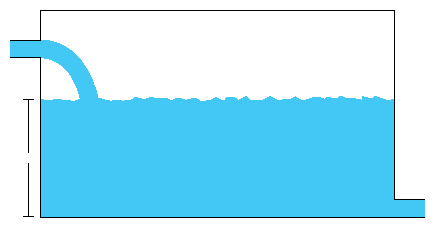
\includegraphics[width=0.7\linewidth]{../../figures/tank-with-hole-no-variables}
\end{center}

What is the \alert{input signal} and \alert{output signal} to the system?
\end{frame}



\begin{frame}[label={sec:orga76c6fa}]{First-order system example: Level control of a tank}
\begin{center}
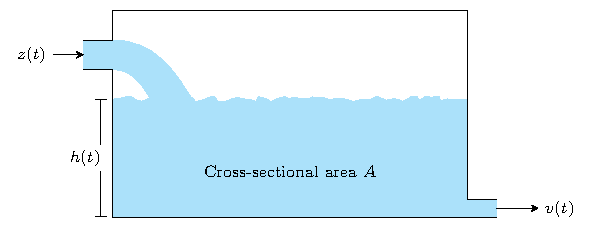
\includegraphics[width=0.7\linewidth]{../../figures/tank-with-hole-simple}
\end{center}

\begin{align*}
\frac{d}{dt} (Ah) &=  z(t) - x(t) = z(t) - a \sqrt{2gh}\quad \Rightarrow\\
\frac{d}{dt} h(t) &= - \frac{a\sqrt{2g}}{A} \sqrt{h(t)} + \frac{1}{A} z(t)
\end{align*}
\end{frame}


\begin{frame}[label={sec:orgeaac400}]{Intuition}
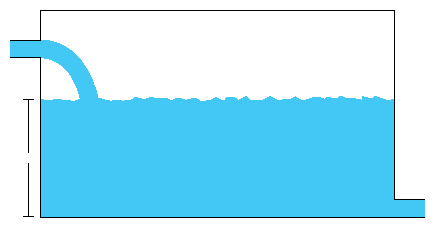
\includegraphics[width=0.2\linewidth]{../../figures/tank-with-hole-no-variables}

\alert{Individual activity} A constant inflow has been present since forever, but at time \(t_1\) the flow in is suddenly shut off. Which of the responses of the water level \(h(t)\) below is correct?

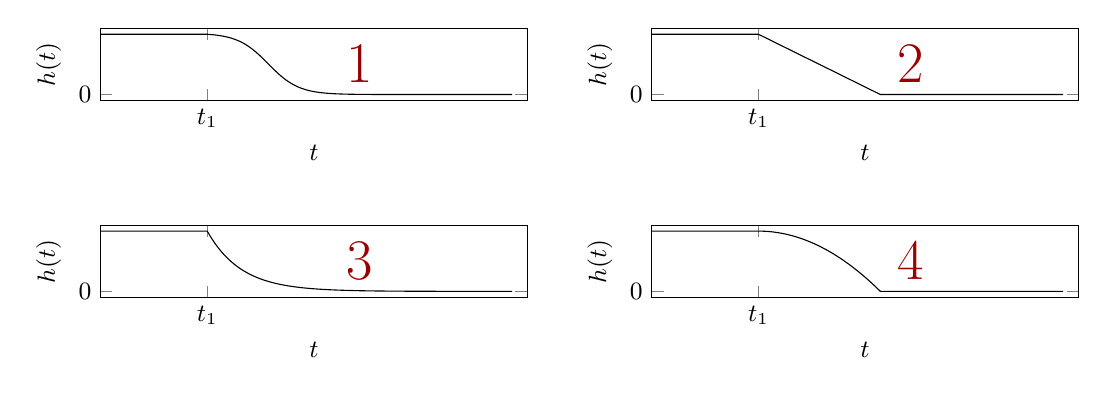
\begin{tikzpicture}
\small

\begin{axis}[
width=7cm,
height=2.5cm,
xlabel={$t$},
ylabel={$h(t)$},
xmin=-3.5,
xmax=10.5,
ytick = {0},
xtick = {0},
xticklabels = {$t_1$},
]
\addplot+[black, no marks, domain=-4:10, samples=400,variable=k] { (k < 0) + (k>0)*(1+exp(-4))/(1+exp(4*(0.5*k-1)))};

\node[black!40!red] at (axis cs: 5, 0.5) {\huge 1};
\end{axis}

\begin{axis}[
xshift=7cm,
width=7cm,
height=2.5cm,
xlabel={$t$},
ylabel={$h(t)$},
xmin=-3.5,
xmax=10.5,
ytick = {0},
xtick = {0},
xticklabels = {$t_1$},
]
\addplot+[black, no marks, domain=-4:10, samples=400,variable=k] { (k<0) + ((k>=0) - (k>4))*(1/4*(4-k)) };
\node[black!40!red] at (axis cs: 5, 0.5) {\huge 2};
\end{axis}

\begin{axis}[
xshift=0cm,
yshift=-2.5cm,
width=7cm,
height=2.5cm,
xlabel={$t$},
ylabel={$h(t)$},
xmin=-3.5,
xmax=10.5,
ytick = {0},
xtick = {0},
xticklabels = {$t_1$},
]
\addplot+[black, no marks, domain=-4:10, samples=400,variable=k] { (k<0) + (k>0)*exp(-0.9*k)};
\node[black!40!red] at (axis cs: 5, 0.5) {\huge 3};
\end{axis}

\begin{axis}[
xshift=7cm,
yshift=-2.5cm,
width=7cm,
height=2.5cm,
xlabel={$t$},
ylabel={$h(t)$},
xmin=-3.5,
xmax=10.5,
ytick = {0},
xtick = {0},
xticklabels = {$t_1$},
]
\addplot+[black, no marks, domain=-4:10, samples=400,variable=k] { (k<0) + ((k>=0) - (k>4))*(1-1/16*pow(-k,2)) };
\node[black!40!red] at (axis cs: 5, 0.5) {\huge 4};
\end{axis}


\end{tikzpicture}
\end{frame}


\begin{frame}[label={sec:orgc81a87f}]{Deviation variables}
\begin{center}
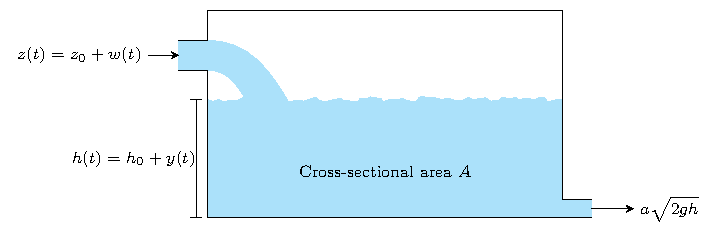
\includegraphics[width=0.7\linewidth]{../../figures/tank-with-hole}
\end{center}

Flow in: \(z(t) = z_0 + w(t)\). Level of water: \(h(t) = h_0 + y(t)\). The constants \(h_0\) and \(z_0\) define an \emph{operating point}.

\begin{align*}
\frac{d}{dt} h(t) &= - \frac{a\sqrt{2g}}{A} \sqrt{h(t)} + \frac{1}{A} z(t)
\end{align*}


\alert{Individual activity} Given \(h_0\) determine the operating point for the inflow, \(z_0\), such that the system is in equilibrium at the operating point.
\end{frame}


\begin{frame}[label={sec:org5f0b24a}]{Intuition}
Which change \(y(t)\) in the water level corresponds to a step change \(w(t)\) in the inflow? 

\begin{center}
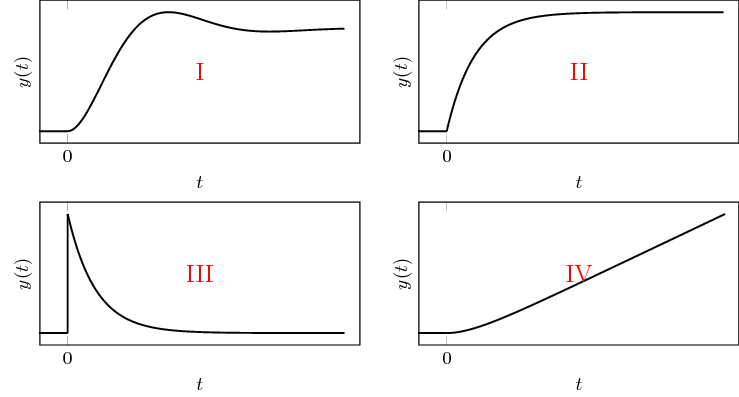
\includegraphics[width=0.7\linewidth]{../../figures/dc-response-exercise}
\end{center}
\end{frame}



\begin{frame}[label={sec:orga6c9c55}]{Fitting a first-order model}
Assuming a plant model of first-order with time-constant \(T\)
\[  \quad \textcolor{green!50!black}{Y(s)} = \frac{K}{sT + 1}\textcolor{blue!80!black}{U(s)} \quad \overset{U(s) = \frac{u_f}{s}}{\Longrightarrow} \quad \textcolor{green!50!black}{y(t)} = u_f K\big( 1 - \mathrm{e}^{-\frac{t}{T}}\big)u_H(t)\]
\def\Tcnst{3}
\def\tdelay{0.0}
\def\ggain{2}
\def\uampl{0.8}
\pgfmathsetmacro{\yfinal}{\uampl*\ggain}
\pgfmathsetmacro{\yone}{0.283*\yfinal}
\pgfmathsetmacro{\ytwo}{0.632*\yfinal}
\pgfmathsetmacro{\tone}{\tdelay + \Tcnst/3}
\pgfmathsetmacro{\two}{\tdelay + \Tcnst}

\begin{center}
  \begin{tikzpicture}
    \begin{axis}[
    width=14cm,
    height=4.5cm,
    grid = both,
    xtick = {0,  \two},
    xticklabels = {0, $T$},
    ytick = {0, \ytwo, \uampl, \yfinal},
    yticklabels = {0,  $ $, $u_f$, $y_f$},
    xmin = -0.2,
    %minor y tick num=9,
    %minor x tick num=9,
    %every major grid/.style={red, opacity=0.5},
    xlabel = {$t$},
    ]
      \addplot [thick, green!50!black, no marks, domain=0:10, samples=100] {\uampl*\ggain*(x>\tdelay)*(1 - exp(-(x-\tdelay)/\Tcnst)} node [coordinate, pos=0.9, pin=-90:{$y(t)$}] {};
      \addplot [const plot, thick, blue!80!black, no marks, domain=-1:10, samples=100] coordinates {(-1,0) (0,0) (0,\uampl) (10,\uampl)} node [coordinate, pos=0.9, pin=-90:{$u(t)$}] {};
    \end{axis}
  \end{tikzpicture}
\end{center}

\alert{Individual activity} Evaluate the response \(y(t)\) at the time instant \(t=T\) and for \(t\to\infty\)!
\end{frame}

\begin{frame}[label={sec:org41c055a}]{Fitting a first-order model}
Assuming a plant model of first-order with time-constant \(T\)
\[  \quad \textcolor{green!50!black}{Y(s)} = \frac{K}{sT + 1}\textcolor{blue!80!black}{U(s)} \quad \overset{U(s) = \frac{u_f}{s}}{\Longrightarrow} \quad \textcolor{green!50!black}{y(t)} = u_f K\big( 1 - \mathrm{e}^{-\frac{t}{T}}\big)u_H(t)\]
\def\Tcnst{3}
\def\tdelay{0.0}
\def\ggain{2}
\def\uampl{0.8}
\pgfmathsetmacro{\yfinal}{\uampl*\ggain}
\pgfmathsetmacro{\yone}{0.283*\yfinal}
\pgfmathsetmacro{\ytwo}{0.632*\yfinal}
\pgfmathsetmacro{\tone}{\tdelay + \Tcnst/3}
\pgfmathsetmacro{\two}{\tdelay + \Tcnst}

\begin{center}
  \small
  \begin{tikzpicture}
    \begin{axis}[
    width=14cm,
    height=3.5cm,
    grid = both,
    xtick = {0,  \two},
    xticklabels = {0, $T$},
    ytick = {0, \ytwo, \uampl, \yfinal},
    yticklabels = {0,  $0.632y_f$, $u_f$, $y_f$},
    xmin = -0.2,
    %minor y tick num=9,
    %minor x tick num=9,
    %every major grid/.style={red, opacity=0.5},
    xlabel = {$t$},
    ]
      \addplot [thick, green!50!black, no marks, domain=0:10, samples=100] {\uampl*\ggain*(x>\tdelay)*(1 - exp(-(x-\tdelay)/\Tcnst)} node [coordinate, pos=0.9, pin=-90:{$y(t)$}] {};
      \addplot [const plot, thick, blue!80!black, no marks, domain=-1:10, samples=100] coordinates {(-1,0) (0,0) (0,\uampl) (10,\uampl)} node [coordinate, pos=0.9, pin=-90:{$u(t)$}] {};
    \end{axis}
  \end{tikzpicture}
\end{center}

\alert{Time-constant:} Find the time \(t=T\) at which the response has reached 63.2\% of its final value

\alert{Gain:} \(y_f = \lim_{t\to\infty}y(t) = Ku_f \quad \Rightarrow \quad K = \frac{y_f}{u_f}\)
\end{frame}

\section{The lab activity}
\label{sec:org6acf095}

\begin{frame}[label={sec:orged6ff34}]{About the tolerance of components and propagation of errors}
\setlength{\tabcolsep}{1cm}

\begin{center}
\begin{tabular}{cc}
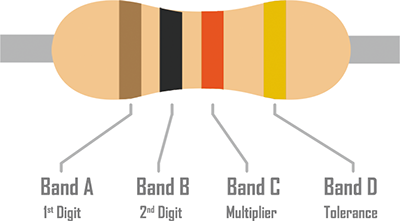
\includegraphics[width=3cm]{../../figures/resistor-color-code-4-band.png} & 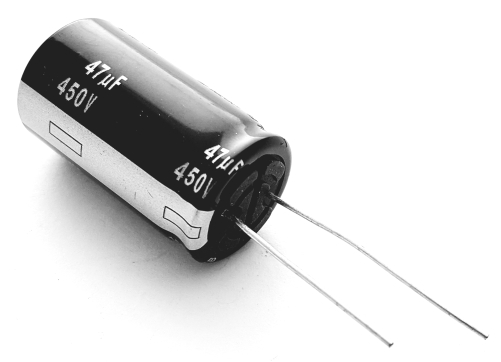
\includegraphics[width=3cm]{../../figures/capacitor.jpg}\\
\(R = R_0 \pm \Delta R\) & \(C = C_0 \pm \Delta C\)\\
\end{tabular}
\end{center}

\[\tau = RC = \tau_0 + \Delta\tau\]

\pause
Assume the tolerance for the resistor is \(\frac{\Delta R}{R_0}=\)5\% and for the capacitor \(\frac{\Delta C}{C_0}=\)20\%. What will the tolerance for the time-constant \(\frac{\Delta\tau}{\tau_0}\) be?
\setlength{\tabcolsep}{1cm}
\begin{center}
\begin{tabular}{cccc}
1. 5\% & 2. 20\% & 3. 25\% & 4. 100\%\\
\end{tabular}
\end{center}
\end{frame}


\begin{frame}[label={sec:org6db2167}]{About the tolerance of components amd propagation of errors}
\small
\begin{columns}
\begin{column}{0.3\columnwidth}
\begin{center}
 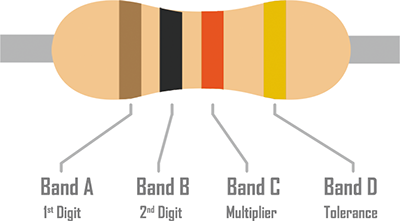
\includegraphics[width=.7\linewidth]{../../figures/resistor-color-code-4-band.png}
\end{center}

\begin{center}
\begin{tabular}{ll}
Color & Meaning\\
\hline
Brown & First digit 1\\
Black & Second digit 0\\
Orange & Multiply with \(10^3\)\\
Gold & Tolerance 5\%\\
\end{tabular}
\end{center}

\begin{align*}
R &= R_0 \pm \Delta R\\
&=10\, \text{k}\Omega \pm 5\% = (10 \pm 0.5)\, \text{k}\Omega
\end{align*}
\end{column}

\begin{column}{0.7\columnwidth}
\[ \tau = RC = R_0C_0 \pm \Delta\tau = \tau_0 \pm \Delta \tau \]

\pause

Two ways to calculate \(\Delta\tau\):
\footnotesize
\begin{enumerate}
\item Direct calculation \begin{align*} \tau &= RC = (R_0 + \Delta R)(C_0 + \Delta C)\\
   &= R_0C_0 + R_0\Delta C  + C_0\Delta R + \Delta R \Delta C\\
   &\approx \tau_0 + \underbrace{R_0\Delta C  + C_0\Delta R}_{\Delta\tau}
   \end{align*}
\item Total derivative \begin{align*} \Delta\tau &= \frac{\partial \tau}{\partial R} \Big|_{R_0, C_0} \Delta R + \frac{\partial \tau}{\partial C} \Big|_{R_0, C_0} \Delta C \\
&=C_0\Delta R + R_0\Delta C.
\end{align*}
\end{enumerate}

\small
\pause
\[\frac{\Delta\tau}{\tau_0} = \frac{C_0\Delta R + R_0\Delta C}{R_0C_0} = \frac{\Delta R}{R_0} + \frac{\Delta C}{C_0}\]
\end{column}
\end{columns}
\end{frame}

\begin{frame}[label={sec:orgd445274}]{About the tolerance of components and propagation of errors}
\setlength{\tabcolsep}{1cm}

\begin{center}
\begin{tabular}{cc}
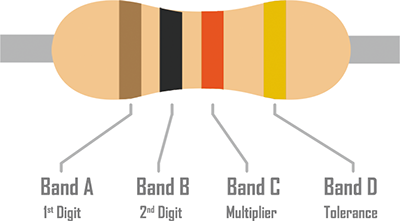
\includegraphics[width=3cm]{../../figures/resistor-color-code-4-band.png} & 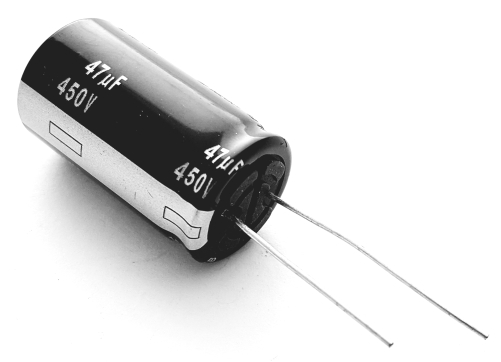
\includegraphics[width=3cm]{../../figures/capacitor.jpg}\\
\(R = R_0 \pm \Delta R\) & \(C = C_0 \pm \Delta C\)\\
\end{tabular}
\end{center}

\[\tau = RC = \tau_0 + \Delta\tau\]

\pause
Assume the tolerance for the resistor is \(\frac{\Delta R}{R_0}=\)5\% and for the capacitor \(\frac{\Delta C}{C_0}=\)20\%. What will the tolerance for the time-constant \(\frac{\Delta\tau}{\tau_0}\) be?
\setlength{\tabcolsep}{1cm}
\begin{center}
\begin{tabular}{cccc}
1. 5\% & 2. 20\% & 3. 25\% & 4. 100\%\\
\end{tabular}
\end{center}
\end{frame}
\end{document}